\begin{figure}[htb!]
    \centering
    \begin{tabular}{cc}
        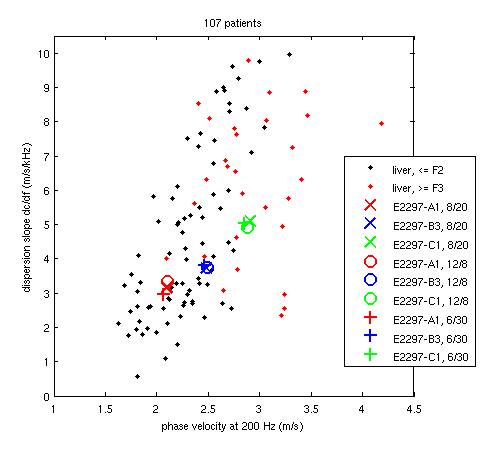
\includegraphics[width=0.5\linewidth]{figs/phantom_liver_scatter_plot.png} &
        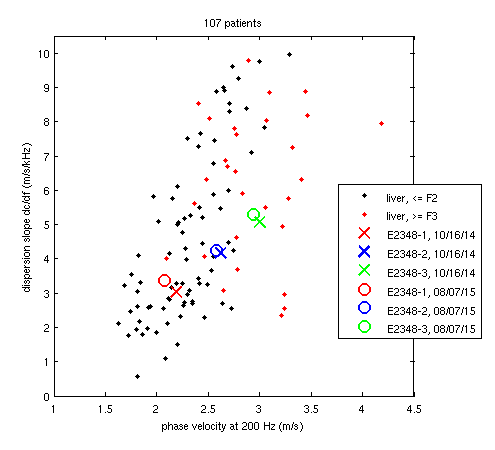
\includegraphics[width=0.5\linewidth]{figs/phaseIIset2scatterplot.png} \\
        (a) CIRS E2297-A1, -B1, -C1 (Phase II, Set 1) &
        (b) CIRS E2348-1, -2, -3 (Phase II, Set 2) \\
    \end{tabular}
    \caption{Scatter plot comparing mechanical properties of liver (black, red
        dots) in 107 patients with measurements from the (a) CIRS E2297-A1,
        B3, and C1 (Phase II, Set 1) phantoms made on August 20, 2014 (X’s),
        December 8, 2014 (O’s), and June 30, 2015 (+’s) and (b) CIRS
        E2348-1, -2, and -3 (Phase II, Set 2) phantoms made on October 16, 2015
        and August 07, 2015, after being shipped to several QIBA imaging sites. 
        Points are plotted as a function of (200 Hz) and $\frac{dc}{df}$ from a
        linear dispersion model from 100--400 Hz.}
\label{fig:phantom_liver_scatter_plot}
\end{figure}
